\section{Grundlagen und Begriffserklärungen}

\subsection{Die Composable-Enterprise-Architektur}

\subsubsection{Begriffserklärung und Abgrenzung}

\subsubsection{Technologische Konzepte des Composable-Enterprises}

\newpage
\subsection{Integration und Bereitstellung von Softwareentwicklungen}


\subsubsection{Agile und DevOps als moderne Anwendungsentwicklungskonzepte}

Das Hauptaugenmerk eines Composable-Enterprises besteht darin, Resilienz und \\Flexibilität aufrechtzuerhalten. Damit soll sichergestellt werden, dass IT-Leistungen in einem sich stetig ändernden Umfeld schnell und risikoarm bereitgestellt werden. Das traditionelle Wasserfallmodell, welches eine sequenzielle Abfolge der Projektelemente \textit{Anforderung}, \textit{Design}, \textit{Implementierung}, \textit{Test} und \textit{Betrieb} vorgibt, besitzt dabei signifikante Limitationen. Die in dieser Methodik detailliert durchgeführte Vorabplanung, kann in der Realität aufgrund unvorhersehbarer Externalitäten selten eingehalten werden. Auch die starre Abfolge der Projektphasen mindert insbesondere in fortgeschrittenen Zeitpunkten des Vorhabens den Spielraum für Anpassungsmöglichkeiten \cite[5]{Vivenzio.2013}. Dies resultiert nicht nur einem Anstieg der Kosten, sondern führt ebenfalls dazu, dass IT-Projekte länger als geplant ausfallen \cite[41]{Vieweg.2015}. Als Reaktion haben sich innerhalb der Projektmanagementlandschaft zunehmend \textbf{agile Vorgehensmodelle} etabliert.
Im Gegensatz zum Wasserfallmodell, welches eine umfassende Vorabplanung vorsieht, wird das Vorhaben in einer agilen Entwicklung in viele Teilprojekte, sog. \textit{Sprints}, segmentiert (s. Abb. \ref*{fig:Agile_Cycle}) \cite[87]{Goll.2015}. 
\begin{center}
	\begin{figure}[H]
		\centering
		\scalebox{0.5}{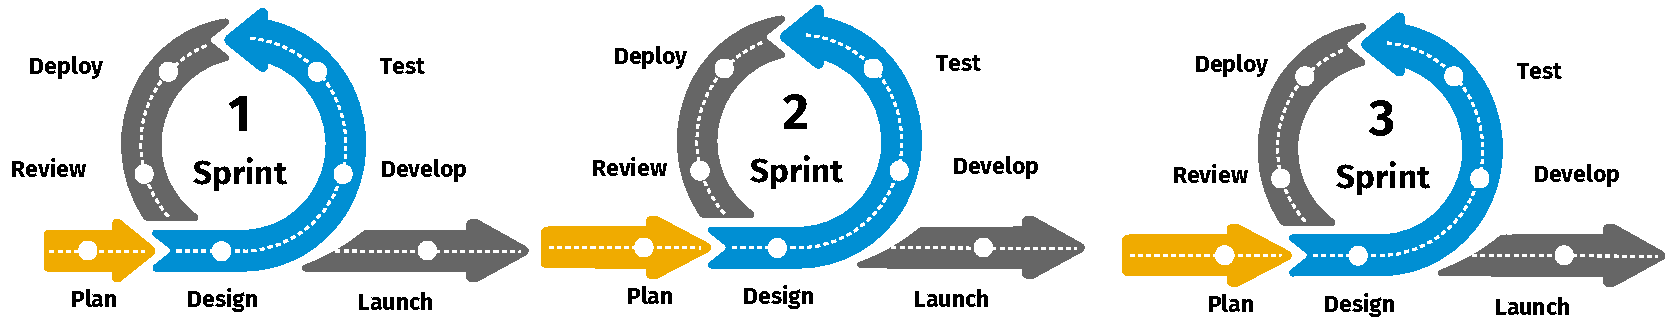
\includegraphics{Agile_Cycle}}
		\caption[Exemplarische Abfolge eines agilen Entwicklungszykluses]{Exemplarische Abfolge eines agilen Entwicklungszykluses. In Anlehnung an K\&C \cite{K&C.2021}.}
		\label{fig:Agile_Cycle}
	\end{figure}	
\end{center}
\vspace*{-15mm}
Sprints sind Durchläufe, welche i.d.R. einen Zeitraum von ein bis vier Wochen umfassen. Während dieses Abschnitts ist die Fertigstellung einer vor dem Teilprojekt definierten Aufgabenkontingente (\textit{Sprint-Backlog}) vorgesehen. Nach Abschluss eines Sprints soll dabei ein potenziell an den Kunden auslieferbares Produkt zur Verfügung gestellt werden. Dies erlaubt eine schnelle Bereitstellung funktionsfähiger Software, was neben der Erhöhung der Kundenzufriedenheit ebenfalls in einer Optimierung der Planungsprozesse resultiert. So kann das nach Ablauf eines Sprints an die Stakeholder ausgelieferte Artefakt als Feedback-Grundlage verwendet und im unmittelbaren Folge-Sprint eingearbeitet werden \cite[39]{K&C.2021}. 
Dieser Sprint-Review-Zyklus wird ausgeführt, bis alle Kundenbedürfnisse erfüllt sind und das Vorhaben als abgeschlossen gilt.
Innerhalb der letzten Dekade haben sich diverse auf agilen Prinzipien basierenden Vorgehensmodelle, wie Scrum, Kanban oder \ac{XP} in der Softwareentwicklung etabliert. Obwohl einige dieser Methoden zur erfolgreichen Zusammenarbeit innerhalb der Entwicklungsteams beigetragen haben, bleibt das sog.  \textit{Problem der letzten Meile} bestehen \cite{Qentelli.20230305}. Traditionell erfolgt eine funktionale Trennung der Entwickler- und IT-Betriebler-Teams. Das Problem der letzten Meile beschreibt dabei, dass aufgrund ausbleibender Kooperation der Entwicklungs- und Betriebsteams der Programmcode nicht auf die Produktivumgebung abgestimmt ist. Erkenntnisse aus der Praxis zeigen, dass solche organisatorischen Silos häufig in einer schlechten Softwarequalität und somit in einem geminderten Ertragspotenzial bzw. in einer Erhöhung der Betriebskosten resultieren \cite[1]{Halstenberg.2020}. So geht aus der von McKinsey veröffentlichen Studie \textit{The Business Value of Design 2019} hervor, dass durchschnittlich 80 Prozent des Unternehmens-IT-Budgets zur Erhaltung des Status quo, also zum Betrieb bestehender Anwendungen verwendet wird. Stattdessen fordert das Beratungshaus eine Rationalisierung der Bereitstellung von Software, um finanzielle Mittel für wertschöpfende Investitionen zu maximieren \cite{.20230305}. Abhilfe schaffen kann das in der Literatur als \textbf{\ac{DevOps}} bekannte Aufbrechen organisatorischer Silos zwischen Entwicklung und dem IT-Betrieb \cite[1]{Halstenberg.2020}. 
Dabei stellt DevOps keine neue Erfindung dar. Stattdessen werden einzelne bereits bewährte Werkzeuge, Praktiken und Methoden, wie z.B. die agile Softwareentwicklung, zu einem umfassenden Rahmenwerk konsolidiert. DevOps zielt dabei auf eine Optimierung des gesamten Applikationslebenszykluses, von Planung bis Bereitstellung der Software, ab. Neben der Bereitstellung von IT-Services umfasst DevOps ebenfalls Aktivitäten zu IT-Sicherheit, Compliance und Risikomanagement. Prägnant zusammenfassen lässt sich das DevOps-Konzept durch das Akronym CAMS: \textit{Culture (Kultur)}, \textit{Automation (Automatisierung)}, \textit{Measurement (Messung)} und \textit{Sharing (Teilen)} \cite[5]{Halstenberg.2020}. Dabei gilt \textit{Kultur} als das wohl wesentlichste DevOps-Erfolgselement. Diese Norm bezweckt eine Kollaborationsmentalität, welche sich über alle Ebenen eines Unternehmens erstreckt. Operative Entscheidungen sollen dabei auf die Fachebenen herunter delegiert werden, welche aufgrund ihrer spezifischen Expertise am geeigneten sind, Dispositionen zu verabschieden \cite[5]{Halstenberg.2020}. Eine \textit{Automatisierung} der Softwarebereitstellungsprozesse ermöglicht, sich wiederholende manuelle Arbeit zu eliminieren. Dies kann ebenfalls zur Rationalisierung und damit zur Senkung der IT-Betriebskosten beitragen. Der dabei erzielte Einfluss wird anhand verschiedener DevOps-Kennzahlen bemessen (\textit{Messung}). Neben der Systemverfügbarkeit und der Instandsetzungszeit ist insbesondere der \textit{Time-to-Market} eine signifikante Metrik \cite[7]{Halstenberg.2020}. 

\begin{center}
	\begin{figure}[H]
		\centering
		\scalebox{0.34}{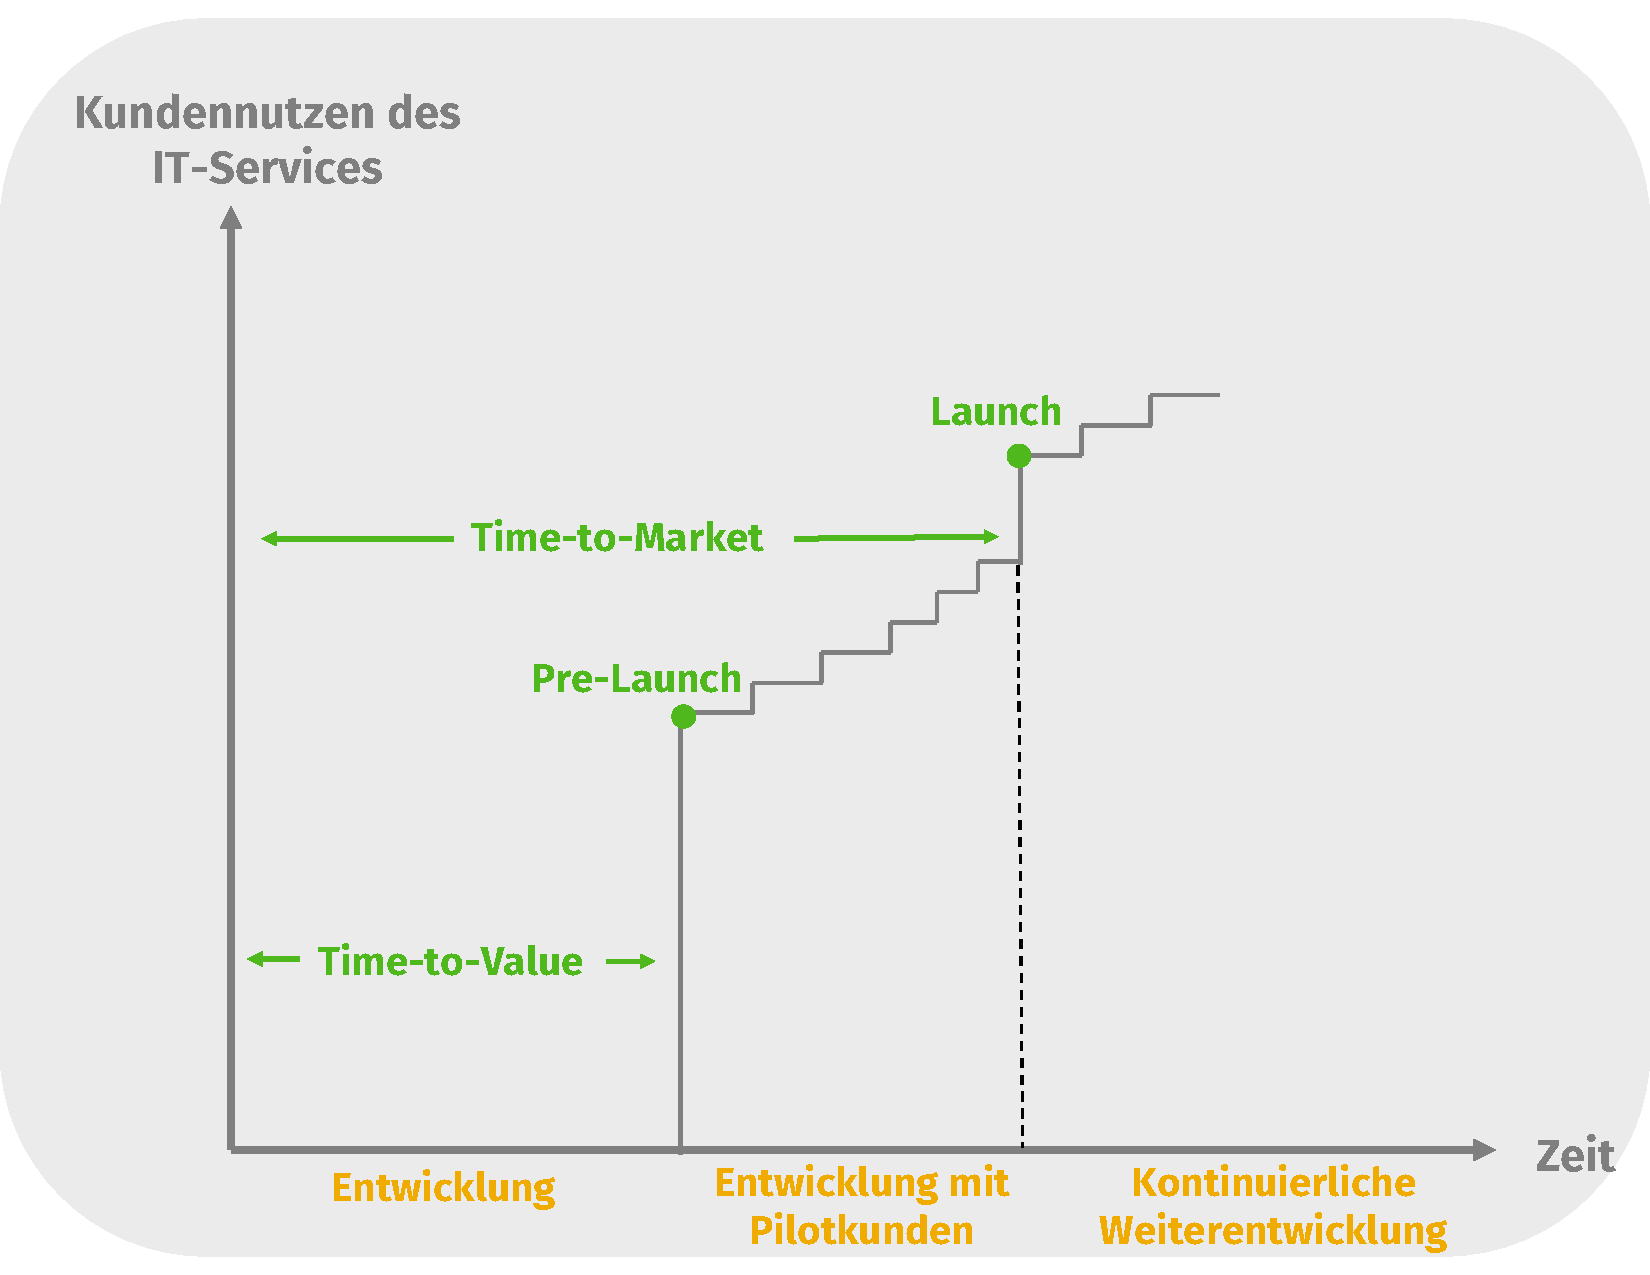
\includegraphics{TTM}}
		\caption[Zeitliche Darstellung des Kundennutzens von IT-Services]{Zeitliche Darstellung des Kundennutzens von IT-Services. In Anlehnung an Halstenberg \cite[9]{Halstenberg.2020}.}
		\label{fig:TTM}
	\end{figure}
\end{center}
\vspace*{-15mm}
Der Time-to-Market beschreibt die Zeitspanne zwischen Entwicklungsentstehungsprozess und der Markteinführung von IT-Services \cite[141]{Vesey.1992}. Auch der \textit{Time-to-Value} erhält zunehmend Bedeutung in der Softwareentwicklung. Im Gegensatz zum Time-to-Market wird hier nicht die Zeit bis zur Komplett-Einführung, sondern bis zum ersten Kundennutzen bemessen. Obwohl der im Time-to-Value bereitgestellte IT-Service möglicherweise Verbesserungspotenzial besitzt, überwiegt der mit der initialen Auslieferung herbeigeführte Mehrwert. Dabei ermöglicht eine solche Früheinführung einen Vorsprung gegenüber Konkurrenten. So ist es dem Softwareunternehmen bereits gelungen, erste Kunden zu akquirieren, deren Input und Feedback möglichst rasch erfasst und verarbeitet werden kann \cite[9]{Halstenberg.2020}. Softwareunternehmen können IT-Services ab dem Pre-Launch somit sukzessive und ressourcenoptimiert unter Zusammenarbeit mit den Pilotkunden erweitern. Auch Adam Caplan, leitender Strategieberater bei Salesforce, empfiehlt angesichts der bei Softwareintegration entstehenden Komplexität, Software schnellst möglichst in Produktivumgebungen zu testen \cite{Vesey.1992}. Aus diesen Erfahrungen sollen Best-Practises entwickelt werden, welche innerhalb von Teams und organisationsübergreifend weitergegeben werden (\textit{Teilen}) \cite[7]{Halstenberg.2020}. 

\subsubsection{Pipelines zur Integrations- und Bereitstellungsautomatisierung}

DevOps beschreibt eine Philosophie zur Förderung der Zusammenarbeit zwischen Entwicklungs- und Betriebsteams. Ein integraler Bestandteil des DevOps-Rahmen\-werks ist \textit{\ac{CI/CD}}. CI/CD ist eine Softwareentwicklungsmethode, welche zur Verbesserung der Qualität bzw. zur Senkung der Entwicklungszeit von IT-Services beitragen soll. Abhilfe schaffen soll dabei eine Pipeline, welche alle Schritte von Code-Integration bis Bereitstellung der Software automatisiert. Hauptaugenmerk liegt dabei auf einer zuverlässigen und kontinuierlichen Bereitstellung von Software \cite[471]{Zampetti.92720211012021}.
\begin{center}
	\begin{figure}[H]
		\centering
		\scalebox{0.5}{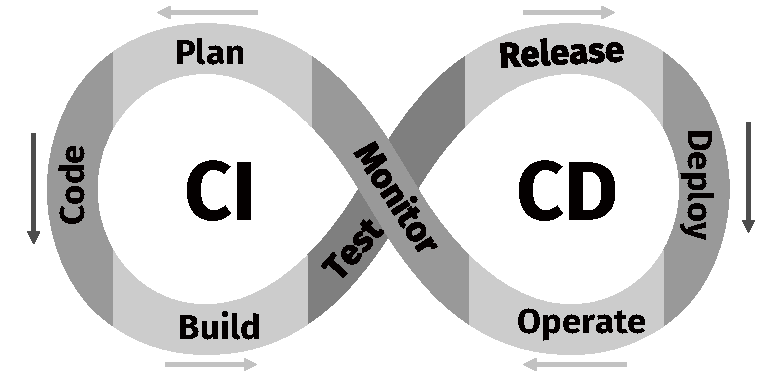
\includegraphics{CICD_Cycle}}
		\captionsetup{format=myformat}
		\caption[Aktivitäten im CI/CD-Prozess]{Aktivitäten im CI/CD-Prozess. In Anlehnung an Synopsys \cite{.20230201}.}
		\label{fig:CICD_Cycle}
	\end{figure}
\end{center}
\vspace*{-15mm}
Alle in diesem Prozess anfallenden Aktivitäten sind dabei dem CI/CD-Zyklus zu entnehmen (s. Abb. \ref*{fig:CICD_Cycle}). Der \acs{CI}-Prozess (Continuous-Integration-Prozess) bezweckt, dass lokale Quellcode\-änderungen in kurzen Intervallen und so schnell wie möglich in eine zentrale Codebasis geladen werden. Das frühzeitige Integrieren von Code soll dabei zu einer unmittelbaren und zuverlässigen Fehlererkennung innerhalb des Entwicklungsvorhabens beitragen \cite[471]{Zampetti.92720211012021}. 
Der erste Schritt des CI-Prozesses umfasst die Planung zu entwickelnder Services (\textit{Plan}: s. Abb. \ref*{fig:CICD_Cycle}). Dabei soll festgestellt werden, welche Anforderungen eine Lösung besitzt bzw. welche Softwarearchitekturen sowie Sicherheitsmaßnahmen implementiert werden sollten. Um sicherzustellen, dass die in der Planung entworfene Anwendungsarchitektur auf das Design des Produktivsystems abgestimmt ist, sollte zu jedem Zeitpunkt das Know-how der Betriebsteams einbezogen werden \cite[16]{Halstenberg.2020}. Nach erfolgreichem Entwurf zu implementierender Anwendungsfeatures beginnt die Entwicklung der IT-Services (\textit{Code}: s. Abb. \ref*{fig:CICD_Cycle}). Arbeiten hierbei mehrere Entwickler parallel an demselben IT-Service, wird der entsprechende Quellcode in sog. \textit{Repositories} wie Github oder Bitbucket ausgelagert. Ein Repository stellt dabei einen zentralen Speicherort dar, welcher das Verfolgen sowie Überprüfen von Änderungen und ein paralleles bzw. konkurrierendes Arbeiten an einer gemeinsamen Codebasis ermöglicht \cite[31]{Loeliger.2012}. Der in dem Repository archivierte Hauptzweig (\textit{Master-Branch}) stellt dabei eine aktuelle und funktionsfähige Version des Codes dar. Dieser mit verschiedenen Validierungsprozessen überprüfte Code, kann dabei zu jeder Zeit in der Produktionsumgebung bereitgestellt werden. (s. Abb. \ref*{fig:VCS}). Im Sinne der agilen Entwicklung werden dabei große Softwareanforderungen, sog. \textit{Epics}, in kleine Features segmentiert, welche in separate Feature-Branches ausgelagert werden. Diese sind unabhängige Kopien des Hauptzweiges, in welcher ein Entwickler Änderungen vornehmen kann, ohne Konflikte in der gemeinsamen Codebasis zu verursachen. Nach Fertigstellung der Funktionalitäten sollte der um die Features erweiterte Quellcode so schnell wie möglich in den Hauptzweig integriert werden. So wird sichergestellt, dass der Code stets stabil, also funktionsfähig ist und keine Konflikte mit dem aktuellen Code des Hauptzweiges aufweist \cite[169]{Loeliger.2012}. Dabei wird eine Validierung des Codes gemäß der \textit{\ac{DoD}} forciert. Die DoD ist eine in der Planungsphase festgelegte Anforderungsspezifikation, deren Erfüllung als notwendige Voraussetzung für den Abschluss eines Features gilt. Im Rahmen dieser Norm sind Entwickler dazu angehalten, für jedes implementierte Feature einen der DoD entsprechenden Test zu entwerfen.
\begin{center}
	\begin{figure}[H]
		\centering
		\scalebox{0.8}{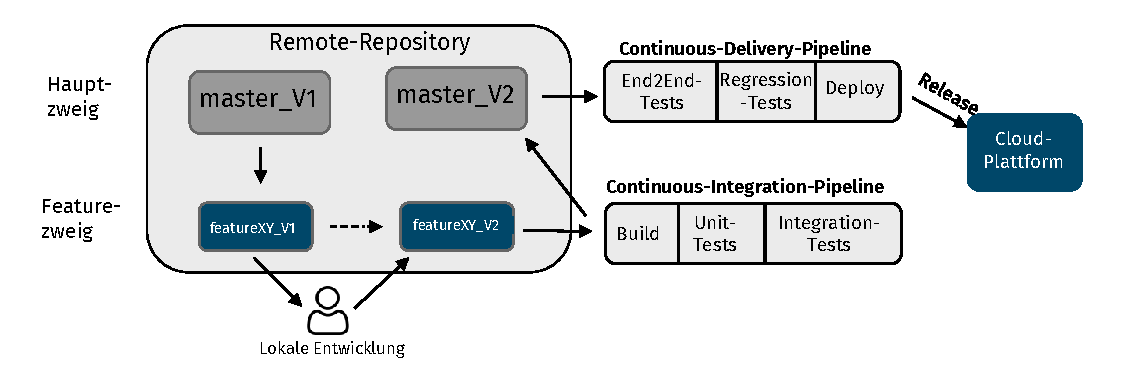
\includegraphics{VCS}}
		\caption[Versionskontrollsysteme zur Verwaltung von Quellcode]{Versionskontrollsysteme zur Verwaltung von Quellcode.\\ Eigene Darstellung.}
		\label{fig:VCS}
	\end{figure}
\end{center}
\vspace*{-10mm}
Die Einbindung des Feature-Branchs in den Hauptzweig resultiert i.d.R. in einem unmittelbaren Start des \textit{CI/CD-Pipeline-Prozesses}. Bei der CI/CD-Pipeline handelt es sich dabei um eine vom Repository unabhängige Recheninstanz, welche auf einer virtuellen Maschine oder in einer containerisierten Computing-Umgebung betrieben wird. Verwaltet wird diese Pipeline entweder von dem Unternehmen selbst (\textit{On-Premise}) oder auf einer externen Cloud-Infrastrukur wie AWS, Azure oder Google Cloud \cite[Kap. 1.2]{Labouardy.2021}. Im ersten Schritt des Pipeline-Prozesses wird die Applikationen zu einem ausführbaren Programm kompiliert (\textit{Artefakt}) anhand welchem verschiedene Tests ausgeführt werden (\textit{Build}: s. Abb. \ref*{fig:CICD_Cycle}). Dafür können je nach Programmiersprache verschiedene Build-Tools, wie Maven für Java oder NPM für Javascript verwendet werden \cite[Kap. 7.1]{Labouardy.2021}. Die dabei durchgeführte Validierung, auch \textit{Smoke-Test}, soll sicherstellen, dass zu jeder Zeit ein rudimentär getesteter Code bereitsteht und grundlegende Funktionalitäten sowie Schnittstellen erwartungsgemäß ausgeführt werden \cite[19]{Halstenberg.2020}. Der in dem Entwicklungszweig bereitgestellte Code wird dabei überwiegend anhand schnell durchführbarer Tests überprüft. Die Abwicklung solcher ressourcenschonender Validierungen hat dabei insbesondere zwei Ursachen. Das Hauptaugenmerk von CI liegt insbesondere in der Realisierung einer hohen Code-Integrationsfrequenz. Aufwendige und langsame Tests würden Entwickler somit hemmen, den Code häufig in dem zentralen Repository bereitzustellen. Des Weiteren soll sichergestellt werden, dass der gesamte lokale Code nicht erst unmittelbar vor Release zusammengeführt wird (\textit{Merge Day}) \cite{.20230308}. Stattdessen sollte der Entwickler ein zeitnahes Feedback auf seine Erweiterungen erhalten, um Fehler und Konflikte so schnell wie möglich entdecken und beheben zu können. Die in der CI-Pipeline abgewickelten Validierungen umfassen i.d.R. \textit{Unit-} sowie \textit{Integration-Tests} \cite[Kap. 1.2]{Labouardy.2021}.
\begin{center}
	\begin{figure}[H]
		\centering
		\scalebox{0.3}{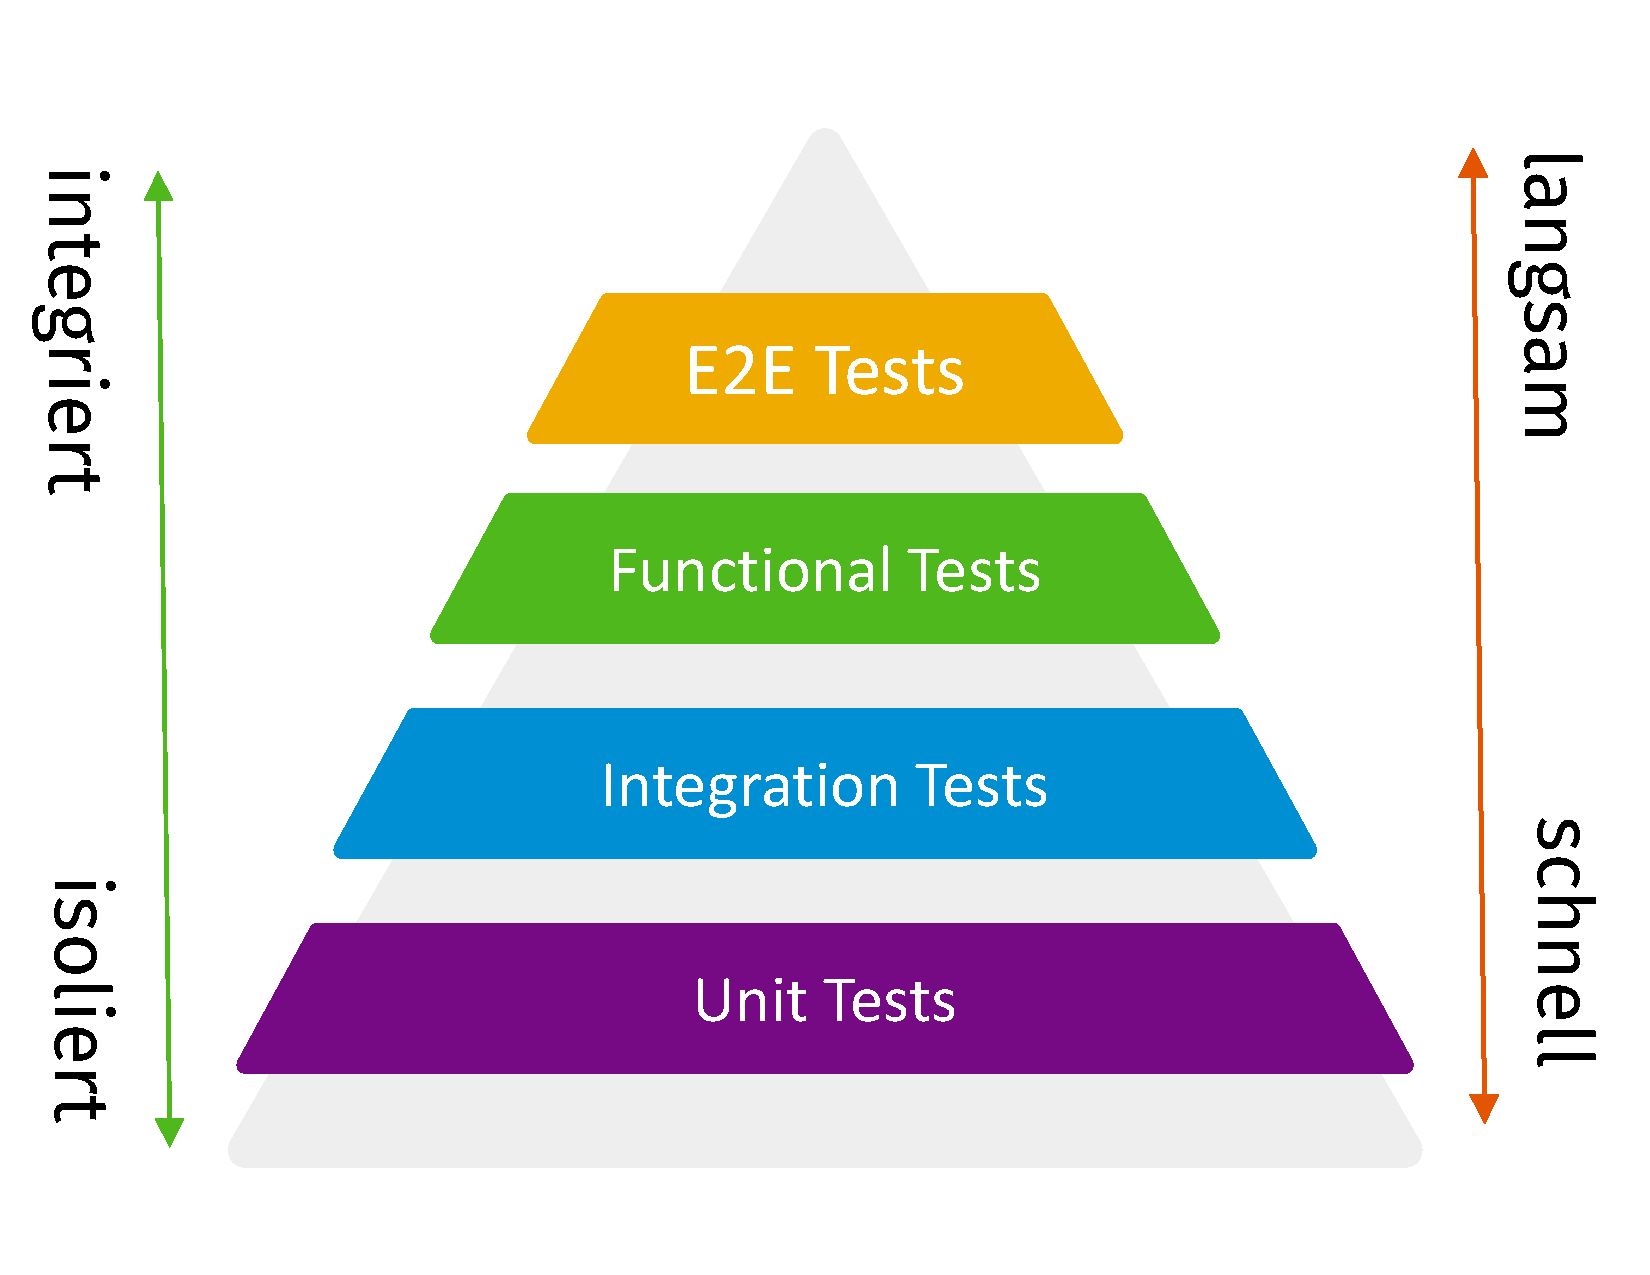
\includegraphics{Tests}}
		\caption[Hierarschische Darstellung von Softwaretests]{Hierarschische Darstellung von Softwaretests.\\ \hspace{0.5cm}In Anlehnung an Paspelava \cite{Exposit.2021}.}
		\label{fig:Tests}
	\end{figure}
\end{center}
\vspace*{-10mm}
Unit-Tests befinden sich dabei auf unterster Hierarchieebene der Test-Pyramide (s. Abb. \ref*{fig:Tests}). Somit besitzen diese eine kurze Ausführungsdauer, werden jedoch ausschließlich in einer isolierten Testumgebung abgewickelt. Mit Unit-Tests wird die funktionale Korrektheit kleinster Einheiten, wie z.B. Methoden einer Klasse, über\-prüft. Der Zweck der Unit-Tests besteht dabei in einer von externen Einflüssen und Daten unabhängigen Überprüfung der einzelnen Komponenten \cite[Kap. 2]{Hambling.2015}. Um bei der Bereitstellung neuer Funktionalitäten ebenfalls das Zusammenspiel verschiedener Komponenten zu überprüfen, werden \textit{Integration-Tests} durchgeführt. Bei diesen Tests können Aspekte, wie der Austausch eines Nachrichtenmodells zweier Web-Services oder das Response-Objekt einer Datenbankabfrage untersucht werden \cite[Kap. 2]{Hambling.2015}. Nachdem einzelne Funktionalitäten entwickelt und alle Tests erfolgreich absolviert wurden, werden die validierten Än\-derungen im Hauptzweig zusammengeführt. Mit diesem Prozessschritt beginnt der \textit{Continuous-Delivery-Workflow (\acs{CD}-Workflow)}.  Während CI den Prozess der kontinuierlichen Integration des Quellcodes in das zentrale Repository verwaltet, steuert der CD-Workflow die Automatisierung der Anwendungsbereitstellung. Applikationen sollen somit ohne große Verzögerungen in die Produktivumgebung und somit zum Kunden ausgeliefert werden. Im Sinne des DevOps-Rahmenwerkes wird der CD-Prozess automatisch und unmittelbar nach Ablauf aller CI-Aktivitäten angestoßen. In der Praxis wird hierbei jedoch häufig ein manueller Schritt zwischengeschalten \cite[20]{Halstenberg.2020}. Damit soll sichergestellt werden, dass das Ausrollen der Anwendung erst nach Überprüfung und Genehmigung aller Entwicklungs-Stakeholder beginnt. Im ersten Schritt des CD-Prozesses wird das in die Produktivumgebung bereitzustellende Artefakt über die Deployment-Pipeline in eine \textit{Staging-Area} geladen. Bei der Staging-Area handelt es sich dabei um ein System, welches zwischen Entwicklungs- und Produktivumgebung liegt. Die Staging-System-Konfigurationen werden dabei so angelegt, dass diese der Produktionsumgebung möglichst ähnlich sind \cite[Kap. 1.3]{Labouardy.2021}. Neben den Datenbanken werden hierbei ebenfalls Serverkonfigurationen, wie Firewall- oder Netzwerkeinstellungen von dem Produktivsystem übernommen. Somit soll sichergestellt werden, dass eine neue Anwendungsversion unter produktions-ähnlichen Bedingungen getestet wird. Analog zum CI-Prozess werden innerhalb des CD-Workflows ebenfalls Unit- und Integration-Tests abgewickelt. Diese sind i.d.R. deutlich rechenintensiver und besitzen längere Ausführungszeiten. Somit werden im CD-Prozess essenzielle, jedoch während des Entwicklungsworkflows zu aufwendige Validierungen durchgeführt \cite[20]{Halstenberg.2020}. In der Staging Area werden unterdessen auch in der Test-Pyramide (s. Abb. \ref*{fig:Tests}) höher positionierte, also rechenintensivere Tests ausgeführt \cite[Kap. 2]{Hambling.2015}. Dazu gehören \textit{Functional-Tests}. Mit diesen werden die in der Planungsphase festgelegten Anforderungen bzw. Funktionen der Anwendung überprüft. So kann z.B. evaluiert werden, ob bei Eingabe einer Benutzer-Passwort-Kennung ein korrekter Autorisierungstoken übergeben wurde. Genau wie bei Integration-Tests wird während Functional-Tests das Zusammenspiel verschiedener Komponenten überprüft. Bei Integration-Tests wird dabei jedoch lediglich die generelle Durchführbarkeit einer Kommunikation verschiedener Komponenten auf Quellcode bzw. Datenbankebene überprüft. Mit Functional-Tests wird darüber hinaus die nach Übermittlung und Prozessierung der verschiedenen Komponenten generierte Ausgabe auf Ebene des Gesamtsystems validiert. Ebenfalls während des CD-Prozesses ausgeführte Validierungen sind \textit{\ac{E2E-Tests}}. Mit diesen soll sichergestellt werden, dass die Anforderungen aller Stakeholder erfüllt werden. Hierbei wird ein vollständiges Anwenderszenario von Anfang bis Ende getestet. Dieses kann im Kontext eines E-Commerce-Webshops etwa das Anmelden mit Benutzername, das Suchen eines Produktes und das Abschließen einer Bestellung umfassen \cite{Bose.20230220}. Nachdem alle Unit-, Integration-, sowie Functional-Tests erfolgreich absolviert wurden, werden i.d.R. verschiedene Codeanalysen angestoßen. Hierbei werden Metriken, wie die prozentuale Testabdeckung oder Schwachstellen verwendeter Code-Patterns überprüft. Nach Durchführung der Codeanalysen wird das überprüfte Artefakt auf die Cloud-Plattform geladen (\textit{Deploy}: s. Abb. \ref*{fig:CICD_Cycle}). Je nach Bereitstellungsstrategie (s. \ref*{sec:Bereitstellungs_Strategien}), wird die Anwendung dann unmittelbar oder erst nach weiteren Überprüfungen für den Kunden zugänglich gemacht. Der letzte Schritt des CD-Workflows umfasst die Laufzeitüberwachung der inbetriebgenommenen Anwendung (\textit{Monitoring}: s. Abb. \ref*{fig:CICD_Cycle}). So soll eine ordnungsgemäße Ausführung der Anwendung in der Produktionsumgebung sichergestellt werden. Wichtige Überwachungselemente sind dabei Infrastruktur- sowie Anwendungs-Monitoring. Beim Infrastruktur-Monitoring werden Metriken wie CPU-, Speicher- und Netzwerklast der Server bzw. Datenbanken untersucht. Das Anwendungs-Moni\-toring umfasst dabei die Überwachung der Funktionalitäten und der Applikation selbst. Hierbei werden Informationen wie Anfragen pro Sekunden, die Anzahl der Benutzer oder die in Log-Dateien gesammelte Fehlercodes analysiert \cite[21]{Halstenberg.2020}. 

\subsubsection{Strategien zur Bereitstellung von Neuentwicklungen}
\label{sec:Bereitstellungs_Strategien}
Nachdem das Artefakt auf der virtuellen Maschine einer Cloud-Instanz installiert und gestartet wurde, entscheiden verschiedene Strategien über die Inbetriebnahme der neuen Softwareversion. Anhand dieser wird festgelegt, mit welcher Methode und zu welchem Zeitpunkt Nutzeranfragen von der aktuellen auf die neue Anwendungsinstanz umgeleitet werden.
\begin{center}
	\begin{figure}[H]
		\centering
		\scalebox{0.4}{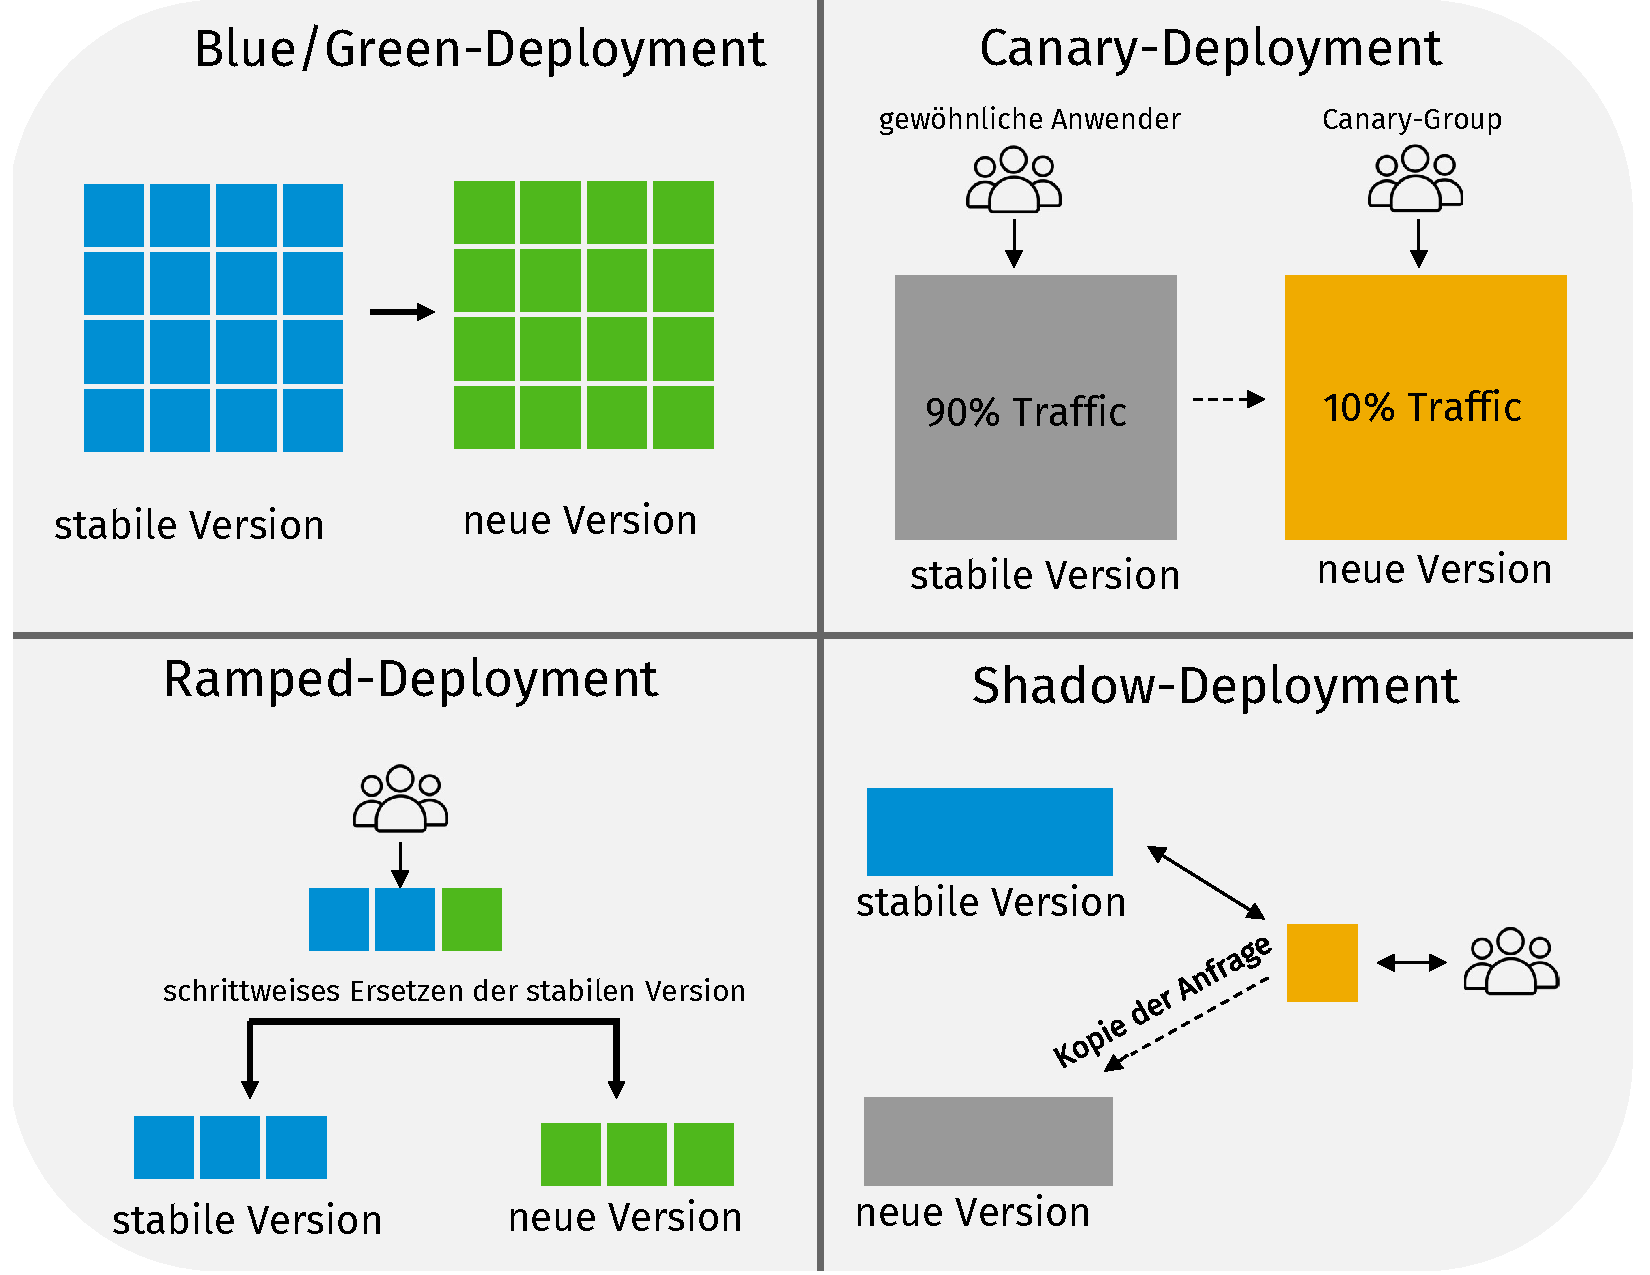
\includegraphics{Deployment_Strategies}}
		\caption[Strategien zur Bereitstellung von Software]{Strategien zur Bereitstellung von Software.\\ In Anlehnung an Ugochi \cite{Ugochi.20220503}.}
		\label{fig:DS}
	\end{figure}
\end{center}
\vspace*{-10mm}
Eine häufig verwendete Deployment-Strategie ist dabei das \textit{Blue/Green-Deployment}. Hierbei wird neben der stabilen aktuellen Anwendung (\textit{Blaue Version}) ebenfalls eine Instanz der neuen Anwendung (\textit{Grüne Version}) betrieben. Nutzeranfragen werden dabei von dem Lastenverteilungsservice (\textit{Load-Balancer}) erst nach Validierung aller Tests umgeschalten. Dazu gehören neben den in der CI/CD-Pipeline definierten Tests ebenfalls Überprüfungen der Qualitätssicherung. Diese umfassen manuelle Tests, in welchen Funktionen, Benutzeroberfläche sowie die Anwenderfreundlichkeit überprüft werden \cite{Ugochi.20220503}. Im Gegensatz zum Blue/Green-Deployment, bei welchem eine neue Version simultan für die gesamte Nutzerbasis zur Verfügung gestellt wird, gewährleistet das \textit{Canary-Deployment} eine restriktivere Nutzlastumleitung. Hierfür wird die neue Anwendungsversion vorerst einer überschaubaren Nutzeranzahl (\textit{Canary-Gruppe}) bereitgestellt. Dabei sollte die zusammengestellte Canary-Gruppe die Gesamtnutzerbasis möglichst gut repräsentieren. Anhand des Canary-Traffics soll der fehlerfreie Betrieb neuer Anwendungen überprüft und ggf. Anpassungen vorgenommen werden, bevor diese der gesamten Nutzerbasis zur Verfügung gestellt werden \cite{Ugochi.20220503}. Für Anwendungen auf einer kritischen IT-Infrastruktur wird i.d.R. die \textit{Ramped-Deployment-Strategie} verwendet. Diese ermöglicht eine präzise Kontrolle horizontal skalierter Services. Die in der horizontalen Skalierung abgewickelte Replizierung von Diensten sorgt für eine höhere Ausfallsicherheit der Anwendungen. Die neue Softwareversion wird während des Ramped-Deployment-Prozesses schrittweise auf die horizontalen Instanzen ausgerollt. Dabei werden die ersten aktualisierten Instanzen lediglich für bestimmte Anwender, eine sog. \textit{Ramped-Gruppe}, bereitgestellt. Dabei soll das von dieser Anwendergruppe zur Verfügung gestellte Feedback während zukünftiger Planungsprozesse berücksichtigt werden \cite{Ugochi.20220503}. Eine aufwendigere, jedoch risikoärmere Bereitstellungsstrategie stellt das \textit{Shadow-Deployment} dar. Dabei wird neben der Instanz der aktuellen Version ebenfalls ein sog. \textit{Shadow-Model} auf der Infrastruktur betrieben. Das Shadow-Model verwaltet die neue Version der Anwendung, kann jedoch nicht unmittelbar von den Nutzern aufgerufen werden. Diese Instanz stellt ein hinter der stabilen Version gelagertes Schattenmodell dar. Benutzeranfragen werden von dem Load-Balancer stets auf die aktuelle Version der Instanz weitergeleitet, verarbeitet und beantwortet. Gleichzeitig wird eine Kopie dieser Anfrage an das Shadow-Model weitergeleitet und von diesem prozessiert. Die Shadow-Modell-Verarbeitung des in der Produktionsumgebung abgewickelten Netzwerkverkehrs ermöglicht den Entwicklern somit eine anwendungsbezogene Überprüfung entwickelter Features \cite{Ugochi.20220503}. 